\section{A Symmetric Scene Reduces the Gap}
\label{sec:symmetry}

The registered symmetric-scene cohort contains 4,096 valid episodes and 2,048 matched pairs across five checkpoint--arena rows. The intervention removes the registered object-layout residual while preserving the robot, camera rig, wrist mounting, reset posture, prompt, seed, and controller. It also uses a registered companion-object inventory transition and is therefore a scene-package intervention, not a position-only edit. Four DROID/RoboLab checkpoints pass the canonical endpoint-redirection positive control and support this comparison. The RoboTwin FastWAM row fails closed and is not used for cross-arena equalization claims. Infrastructure-invalid attempts remain outside behavioral denominators. The powered $\pi_{0.5}$ endpoint uses seeds 9400--9740 and is independent of C002, whose 341 blocks use seeds 12000--12340.

\begin{figure*}[t]
  \centering
  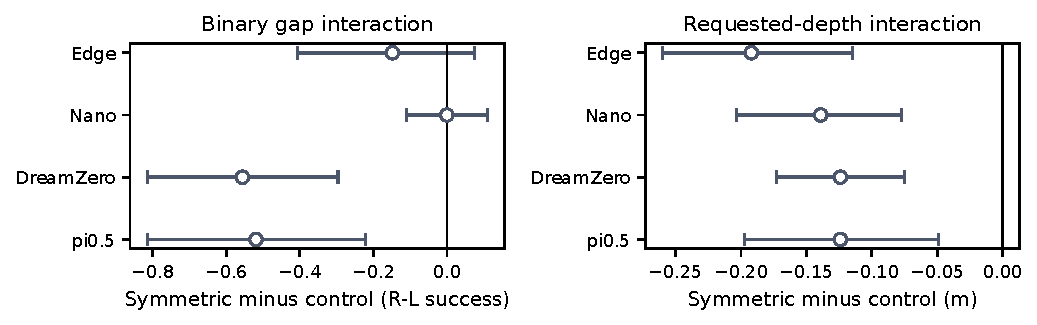
\includegraphics[width=0.98\textwidth]{figures/symmetry_core.pdf}
  \caption{\textbf{The registered symmetric scene reduces directional disparity in the positive-control-passing DROID/RoboLab cohort.}
  Points show symmetric-minus-control interactions in the matched 27-seed core, with seed-clustered 95\% intervals. Requested-depth disparity decreases in every checkpoint. Binary interaction is compressed where the control policy is already at ceiling, as for Nano.}
  \label{fig:symmetry}
\end{figure*}

For $\pi_{0.5}$, the full 341-seed endpoints show the binary RIGHT-minus-LEFT gap falling from 74.2 to 20.2 percentage points and the requested-depth gap from 17.0 to 5.75\,cm. At the symmetric endpoint, their paired 90\% intervals are $[15.0,25.2]$ points against a registered $\pm15.56$-point margin and $[4.85,6.66]$\,cm against $\pm4.15$\,cm; neither is equivalent. The separately defined matched 27-seed core estimates interactions of $-51.9$ points (95\% CI $[-81.5,-22.2]$, $p=.00786$) and $-12.4$\,cm (95\% CI $[-19.7,-4.9]$, $p=.00348$), respectively. Canonical redirection at the symmetric endpoint is $+23.9$\,cm, with $335/341$ positive pairs. The larger sample estimates that endpoint, while the matched core supplies the scene-intervention test.

The matched core also shows why no single summary suffices. DreamZero's observed binary gap changes from $+51.9$ to $-3.7$ points (interaction $-55.6$ points, $p=.00085$), bringing the measured gap near zero without establishing equivalence. Nano has exactly zero binary interaction at ceiling ($p=1$), yet its 27-seed depth interaction is $-13.9$\,cm ($p=1.8\times10^{-4}$). Cosmos3 Edge is underpowered for its $-14.8$-point binary interaction, while its depth interaction is $-19.2$\,cm (95\% CI $[-26.0,-11.5]$). Fig.~\ref{fig:symmetry} keeps these estimands separate.

\begin{figure}[t]
  \centering
  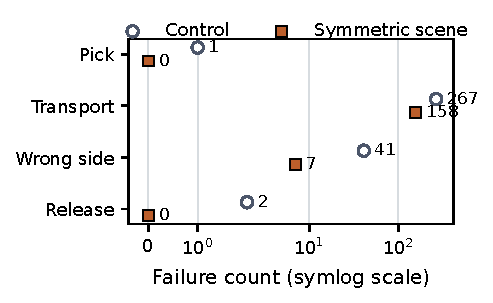
\includegraphics[width=0.98\columnwidth]{figures/failure_composition.pdf}
  \caption{\textbf{$\pi_{0.5}$ failure composition shifts in the matched E004 cohort.}
  Counts pool directions over 341 matched seed pairs (682 episodes per scene). All registered failure categories, including release, are retained. The plot is descriptive; it does not localize an internal policy mechanism.}
  \label{fig:failures}
\end{figure}

The same intervention changes failure composition (Fig.~\ref{fig:failures}). Transport failures fall from 267 to 158, wrong-side failures from 41 to 7, pick failures from 1 to 0, and release failures from 2 to 0. Thus the scene package improves manipulation outcomes without changing the policy or prompt.
